\section{ПРОЕКТИРОВАНИЕ ПРОГРАММНОГО КОМПЛЕКСА}

Важным этапом разработки любого программного комплекса является его проектирование. Любой проект, связанный с созданием программного продукта, требует предварительного проектирования, построения структуры и планирования сроков разработки. После предварительного утверждения плана разработки и выбора используемых технологий и структуры программного продукта начинается его реализация.

В данном разеделе будет произведен анализ основных требований; рассмотрены этапы проектирования основных модулей системы.

\subsection{Анализ требований и постановка задачи}

Разработанный программный прогаммный комплекс по управлению централизованными продажами в системе Bycard должен предоставить единый интерфейс для покупки билетов на мероприятия. Это значительно облегчит разработку клиентов для продажи билетов: мобильных приложений, сайта.

Система должна аггрегировать актуальную информацию о проходящих мероприятиях: расписание, цены на билеты, наличие доступных для продажи мест, возможность покупки билета онлайн. А также предоставить информационными ресурсам удобный механизм интерграции, благодаря которому будет возможность размещать актуальную афишу мероприятий на сторонних сайтах, показывать кнопки для покупки билета.

Большое значение имеют затраты на подключение к системе группы новых объектов, синхронизации данных между ними. Необходимо разработать механизм, который позволит подключать к системе объекты для продажи билетов с минимальными затратами.

\subsection{API}

Один из главных модулей системы. В данном разделе приводится его описание. Затронуты вопросы о стабильности и надежности работы всей системы в целом. Описаны механизмы, которые позволяют балансировать нагрузку на внешних подсистемах.

\subsubsection{Структура}

Данный модуль системы предоставляет общий интерфейс для общения с объектами, подключёнными к системе. Объекты могут иметь различные интерфейсы обмена данными. Например, система для продажи билетов, установленная в кинотеатре наверняка отличается от той, что установлена в театрах, филармонии, концертных залах и т.д. Поэтому логично будет написать для каждой группы объектов отдельный клиент, который будет необходимый интерфейс методов. Для кинотеатров это будет одна реализация, для театров - другая. Обобщённая структура изображена на рисунке ~\ref{fig:api-struct}:

\begin{figure}[H]
  	\centering
 	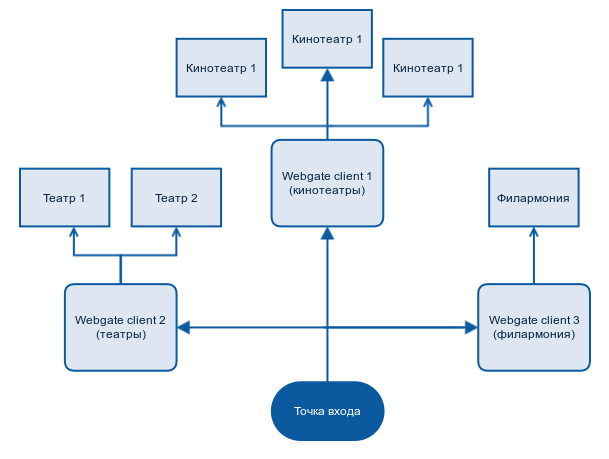
\includegraphics[width=1\textwidth]{images/api-struct.png}
  	\caption{Структура API}
    \label{fig:api-struct}
\end{figure}


В терминах проекта будем далее называть объект, подключенный к системе вебгейтом, а клиент для работы с ним - вебгейт-клиентом. Каждый клиент для вебгейта должен реализовывать необходимый минимум методов, определенных в интерфейсе WebgateClientInterface. Это методы для для реализации фукнции покупки билета: метод блокировки и разблокировки места, создания и отмены заказа. Метод getOrder используется в чекере, который будет описан дальше. Метод getPerformances нужен для получения списка мероприятий, цен на события, которые проходят в конкретном объекте. Система с заданной периодичностью получает актуальную информацию, обновляет её и сохраняет для дальнейшего использования. Приведем список основных методов интерфейса:


\begin{itemize}
    \item getPerformances();
	\item authorize();
	\item lockPlace();
	\item unlockPlace();
	\item createOrder();
	\item cancelOrder();
	\item unlockPlaces();
	\item getPlaces();
	\item addPayment();
	\item returnPlace();
	\item getOrder();
\end{itemize}


\subsubsection{Обработка запроса}

Одна из основных задач системы снизить нагрузку на конечные вебгейты. Для этого разработан механизм отложенных запросов. Согласно этому механизму некоторые запросы не обязательно выполять сразу. В данном случае запрос помещается в очередь отложенных запросов. Запросы из очереди выполняются с задержкой, в зависимости от загруженности конечно вебгейта. Данный механизм позволяет значительно снизить загруженность сервера на объекте. Алгоритм обработки запроса к апи приведен на рисунке ~\ref{fig:request-timeline}:

\begin{figure}[H]
  	\centering
 	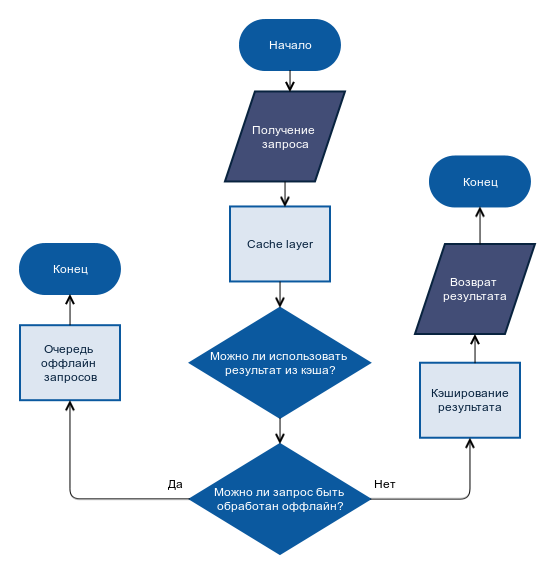
\includegraphics[width=1\textwidth]{images/request-timeline.png}
  	\caption{Алгоритм обработки запроса к API}
    \label{fig:request-timeline}
\end{figure}

Обработчик очереди запросов работает отдельно для каждого из вебгейта. На очередной итерации выбирается еще не выполненный запрос и делается попытка его выполнить. Если запрос выполнен, успешно и вернулся корректный ответ по нему, то он помечается как выполненный. Выполненные запросы в дальнейшем никак не обрабатывается. Однако возможен вариант, при котором запрос выполнился некорекктно, либо мы система не получила корректного ответа по нему, и не известно, отработал он на вебгейта или нет. В данном случае запрос будет обработан повторно через некоторое время либо снят из очереди по истечении количества попыток или потере актуальности. Данный механизм возможен и для онлайн-запросов, который сразу не попадают в очередь отложенных. Если онлайн-запрос не отработал корректно, но его выполнение критично - он может быть помещен в очередь отложенных запросов. После этого его обработка будет проходить по схеме, изложенной выше.

Важным дополнением к задаче является кэширующий слой. Большинство запросов, связанных с получением данных, можно кэшировать на определенный период. В данном случае запрос на конечный вебгейт не посылается вовсе, а данные берутся из кэша системы. Отметим одно из самых частых обращений к апи - запрос на получение карты. Его можно кэшировать на небольшой промежуток времени.


\subsubsection{Интеграция с информационными ресурсами}

Одной из задач системы является аггрегирование актуальной афиши мероприятий. Это даёт возможность делиться данной информацией с различными информационными ресурсами. Многие ресурсы размещают у себя афишу кино, театров и других развлекательных мероприятий. Упрощённая схема взаимодействия показана на рисунке ~\ref{fig:ir-schema}

\begin{figure}[H]
  	\centering
 	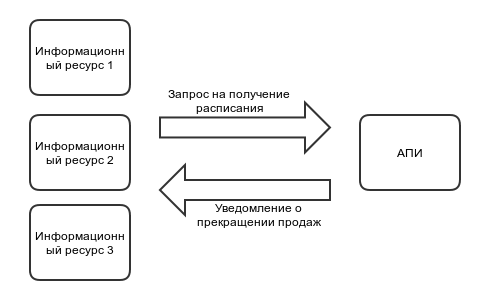
\includegraphics[width=1\textwidth]{images/ir-schema.png}
  	\caption{Упрощенная схема взаимодействия с информационными ресурсами}
    \label{fig:ir-schema}
\end{figure}

API предоставляет возможность выгрузить расписание полностью. С другой стороны хорошо иметь возможность не выгружать всё полностью каждый раз, а получать только обновления. Для этого реализован метод, который позволяет получить все обновления после определенного времени, которое задаст информационный ресурс.

Также есть возможность посылать уведомления со стороны системы о каких-либо изменениях. Например о том, что все билеты на какой-либо сеанс проданы. Информационный ресурс при желании может их тоже обрабатывать.

\subsection{Мониторинг работоспособности}

Через систему каждый день проходит большое количество операций по покупке билетов. Для большой системы, в которой есть большое количество независимых подсистем, необходим механизм который бы автоматически проверял работоспособность и корректную работу подсистем и, в случае найденной неисправности, пытался в автоматическом режиме исправить проблему, либо, при невозможности автоматического восстановления работы, посылал сигнал оператору, который пытается уже решить проблему в ручном режиме.

Мониторинг рабоспособности билетных операций - одна из важных задач. На рисунке ~\ref{fig:checker.png} изображен алгоритм работы чекера заказов. Рассмотрим его в качестве примера

\begin{figure}[H]
  	\centering
 	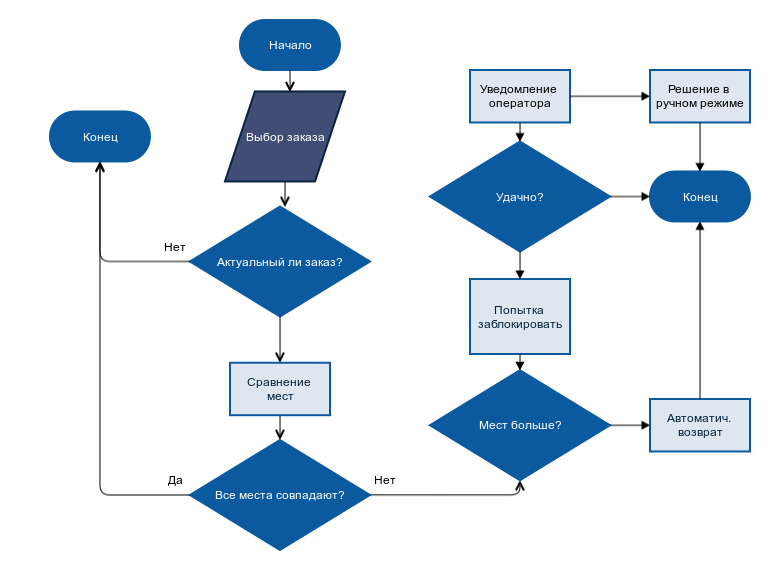
\includegraphics[width=1\textwidth]{images/checker.png}
  	\caption{Алгоритм работы чекера}
    \label{fig:checker.png}
\end{figure}

Выбирается очередной, еще не проверенный заказ. Для каждого билета в заказе делается проверка на то, что данный билет существует в базе конечного вебгейта, который чаще всего расположен в месте проведения мероприятия. Проверяется соотвествие мест, цена, дата и время сеанса. Если информация совпадает - алгоритм заканчивает работу над текущим заказом и переходит к следующему. Иначе делается попытка исправить данные в вебгейте в автоматическом режим, чтобы информация на билете совпадала с информацией из вебгейта. Если в итоге не получается решить проблему, заказ помечается соответсвующей меткой, и переходит к оператору. При любом варианте далее заказ отправляется на повторную проверку до момента, пока чекер не скажет, что он полностью корректный.

Таким образом обеспечивается корректность работы билетных операций, уменьшается риск возникновения непредвиденных ситуаций. Так как операции преимущественно выполняется в автоматическом режиме, уменьшается риск человеческой ошибки. 


Кроме чекера заказов в билетных операциях в системе есть чекеры работоспособности вебгейтов и других подсистем, таких как инфокиоски для доставки билетов и т.д.
Постоянный мониторинг в автоматическом режиме способствуют надёжной работе всей системы в целом.


\subsection{Панель мониторинга оператора}


Панель мониторинга и соответствующие ей веб-части содержат большое количество полезных данных о ходе продаж, статистике и качестве работы всех подсистем. Поскольку панель  постоянно подключена к источникам данных, сведения в ней своевременно обновляются и, как правило, являются интерактивными.

Панель мониторинга оператора предназначена для просмотра статистики, мониторинга работоспособности подсистем в ручном режиме. Как уже было отмечено, в ней отображаются  задачи которые не удалось решить автоматической системе. Схема того, как оператор взаимодействует с автоматической системой представлена на рисунке ~\ref{fig:panel.png}

\begin{figure}[H]
  	\centering
 	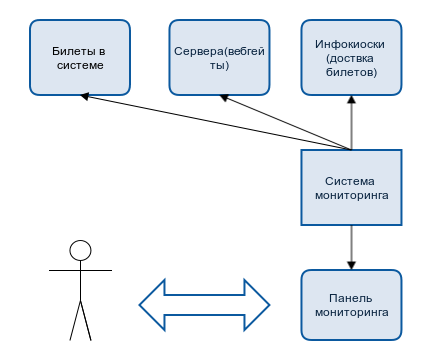
\includegraphics[width=1\textwidth]{images/panel.png}
  	\caption{Панель мониторинга оператора}
    \label{fig:panel.png}
\end{figure}

Также панель мониторинга поддерживают следующие возможности:

\begin{itemize}
	\item изменение уровня детализации данных;
    \item поиск нужных данных путем фильтрации;
    \item изучение данных с помощью действий в различных меню;
    \item формирование отчетов;
    \item экспорт отчетов;
	\item просмотр статистики.
\end{itemize}

Здесь могут быть представлены отчеты самых разных типов, каждый из которых выполняет определенную задачу. Некоторые отчеты формируются из сведений о продажах на стороне API, другие - из сведений на стороне платежных систем, третьи - из сведений на стороне вебгейтов. Также существует механизм сверки отчетности, который при правильной настройке сообщает о проблемах, связанных с различиями в отчетах.


















\newpage